% =============================================================================
% COPYRIGHT AND DISCLAIMER
% =============================================================================
% This file is provided as a convenience template for competition participants.
% By using it, you accept full responsibility for compliance with all applicable
% copyright, licensing, and usage rules of the Association for Computing
% Machinery (ACM) and of any LaTeX packages you load (including, without
% limitation, the "acmart" document class and related ACM materials).
%
% Consult ACM's official publication, template, and copyright policies before
% using this setup for any purpose other than this competition. Do not assume
% that this template may be reused, redistributed, or submitted elsewhere
% without independently verifying ACM's current rules.
%
% Use of the "acmart" class, the "sigconf" option, or ACM-style formatting in
% this template does NOT mean that this report, this competition, its organizers,
% or any resulting PDF is sponsored, endorsed, affiliated with, or published by
% ACM. ACM trademarks and branding remain the property of ACM.
%
% Template packages live in preamble.tex.
% Citations live in main.bib. Edit this file with your paper content.
% =============================================================================

\documentclass[sigconf]{acmart}
\input{preamble}

% Guide styling: \guideStyletrue = show gray italic hints; \guideStylefalse = omit them
% \guideStyletrue
\guideStylefalse

\begin{document}

\title{Where Filament Segmentation Fails: Model Errors Concentrate on Filaments the Annotators Disagree On}
\subtitle{A Solution to the Solar Filament Segmentation Challenge 2026} % DO NOT CHANGE


\author{Saifuddin}
\affiliation{%
  \country{TODO}  % <- TODO: your country
}
\email{TODO@example.com}   % <- TODO: replace with your own email

\begin{abstract}
    This report describes our solution to the Solar Filament Segmentation Challenge~2026, a Kaggle competition on automatic segmentation of solar filaments in GONG H-$\alpha$ observations. Our pipeline detects filaments with two YOLO11s detectors running at 1280 and 1920~px, fuses their boxes, turns each box into a mask with a box-seeded ResNet34 U-Net, and assembles strictly non-overlapping instances. It reaches a Panoptic Quality (PQ) of 0.444 (95\% CI 0.419--0.467) on held-out training observations and 0.39 on the public leaderboard, and the repository reproduces the submitted file byte-for-byte from the included weights. Our main finding concerns the labels rather than the model: on held-out observations with several annotators, the model finds 84\% of the filaments that every annotator marked but only 34\% of those marked by a single annotator, and 53\% of its ``false positives'' with respect to one annotator were drawn by another. Two annotators of the same image agree with each other at a PQ of only 0.33. Six further detector and refiner variants all landed between 0.42 and 0.45, consistent with label ambiguity, not model capacity, limiting the score.
\end{abstract}

\maketitle

\ifguideStyle
\noindent{\color{gray!65}\itshape
Guide mode is on.}
\par\medskip
\fi


% ==================================== %
%              INTRODUCTION            %
% ==================================== %
\section{Introduction}
    This report goes over the details of our submitted solution to the Solar Filament Segmentation Challenge~2026 \cite{filament-segmentation-2026}. The challenge, launched on July~10,~2026, is organized by the Earth-Space AI Research (ESAIR) Lab\footnote{\href{https://www.esairlab.com/home}{www.esairlab.com/}}. This challenge utilizes the MAGFiLO dataset for evaluation of the segmentation algorithms \cite{ahmadzadeh2024dataset}.

    We contribute (i) a two-stage detect-then-refine pipeline whose every reported number is reproducible from a public repository\footnote{\url{https://github.com/syehsyoh-dokling/filament-solution}} (code, weights, notebook), and (ii) an error analysis on held-out training observations showing that most remaining errors fall on filaments whose very existence the expert annotators disagree on. We report negative results as well, because they are what support the second point.


% ==================================== %
%              METHODOLOGY             %
% ==================================== %
\section{Methodology}\label{sec:methodology}

\begin{figure*}[t]
  \centering
  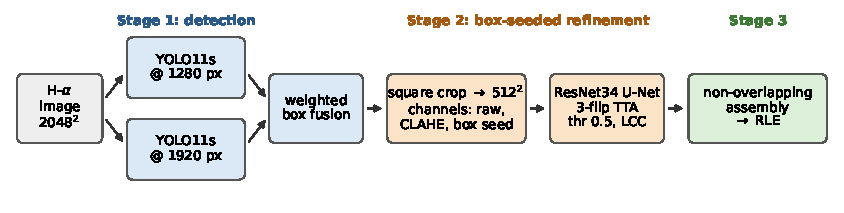
\includegraphics[width=\textwidth]{fig_pipeline.pdf}
  \vspace{-6mm}
  \caption{End-to-end pipeline. Stage~1 proposes boxes with two detectors and fuses them; Stage~2 segments one filament per box from a crop plus a box ``seed''; Stage~3 resolves overlaps and writes COCO RLE.}
  \label{fig:pipeline}
\end{figure*}

\subsection{Pipeline}
Figure~\ref{fig:pipeline} shows the pipeline; all settings are in one configuration file of the repository.

\textbf{Pre-processing.} Each observation is read as a 2048$\times$2048 grayscale image. No other pre-processing is applied to the full image; contrast enhancement happens per crop in Stage~2.

\textbf{Stage 1: detection.} Two YOLO11s detectors \cite{yolo11} (COCO-pretrained, fine-tuned on filament boxes) run at input sizes 1280 and 1920~px and keep boxes with confidence $\geq$0.05 (NMS IoU 0.5). Their boxes are merged by weighted box fusion \cite{solovyev2021wbf}: boxes are visited by decreasing confidence; a box joins the best-overlapping cluster (IoU $>$0.55) that holds no box of the same detector, the cluster box is the confidence-weighted mean of its members, and its score is the sum of member confidences divided by the number of detectors, so a box seen by only one detector is down-weighted.

\textbf{Stage 2: box-seeded refinement.} For each fused box we take a square window of 1.5$\times$ the longer box side (at least 96~px), shifted to stay inside the image, and resize it to 512$\times$512. A U-Net \cite{ronneberger2015unet} with an ImageNet ResNet34 encoder \cite{he2016resnet,iakubovskii2019smp} receives three channels: the crop, its CLAHE-enhanced copy \cite{zuiderveld1994clahe} (clip 2.0, 8$\times$8 tiles), and a filled box seed padded by 60\% of the box size, which tells the network \emph{which} filament in the crop to segment. Probabilities are averaged over the identity, horizontal-flip and vertical-flip inputs, upsampled to native resolution with linear interpolation, thresholded at 0.5, and reduced to the largest connected component.

\textbf{Stage 3: instance assembly.} Masks are visited by decreasing fused score down to 0.32. Pixels already claimed by a stronger instance are removed, so the output never contains overlapping instances, and remnants under 200~px are dropped. An observation with no box above 0.32 keeps its single best candidate.

\textbf{Efficiency.} The 180 test observations take 266~s on one Tesla T4 (1.5~s per observation, all three models, TTA included); the three weight files total 130~MB.

\subsection{Training data, sampling and splits}
We use only the competition training set: 707 observations with one or more annotator passes each, and only their segmentation masks. The detector targets are the boxes stored with each annotation, which coincide with the tight boxes of the masks (99.2\% within 2~px, median difference 0.5~px); the spine and chirality fields are never used. We split by \emph{observation} (seed 42, 15\%), so all passes of an image fall on the same side: 601 observations for training, 106 (170 annotator passes, 1{,}258 filaments) held out. All three models were trained on the same split.

The detectors use the Ultralytics default augmentation (40 epochs at 1280~px and 60 epochs at 1920~px). The refiner is trained on one crop per annotated filament for 12 epochs (AdamW, lr $3\cdot10^{-4}$, cosine schedule, loss 0.45~BCE + 0.55~soft Dice). To make the training seed look like a detector box, the ground-truth box is randomly shifted ($\pm$15\%), rescaled (0.85--1.25) and padded (30--90\%), with random flips. Checkpoints were selected on held-out Dice/mAP and the score threshold on held-out PQ, so held-out numbers are mildly optimistic; the public leaderboard is the unbiased estimate.

\subsection{Examples}
Figure~\ref{fig:examples} shows two held-out observations that each have two annotator passes, next to our prediction. The two annotators disagree on about half of the filaments; our prediction has as many instances as the more conservative annotator.

\begin{figure*}[t]
  \centering
  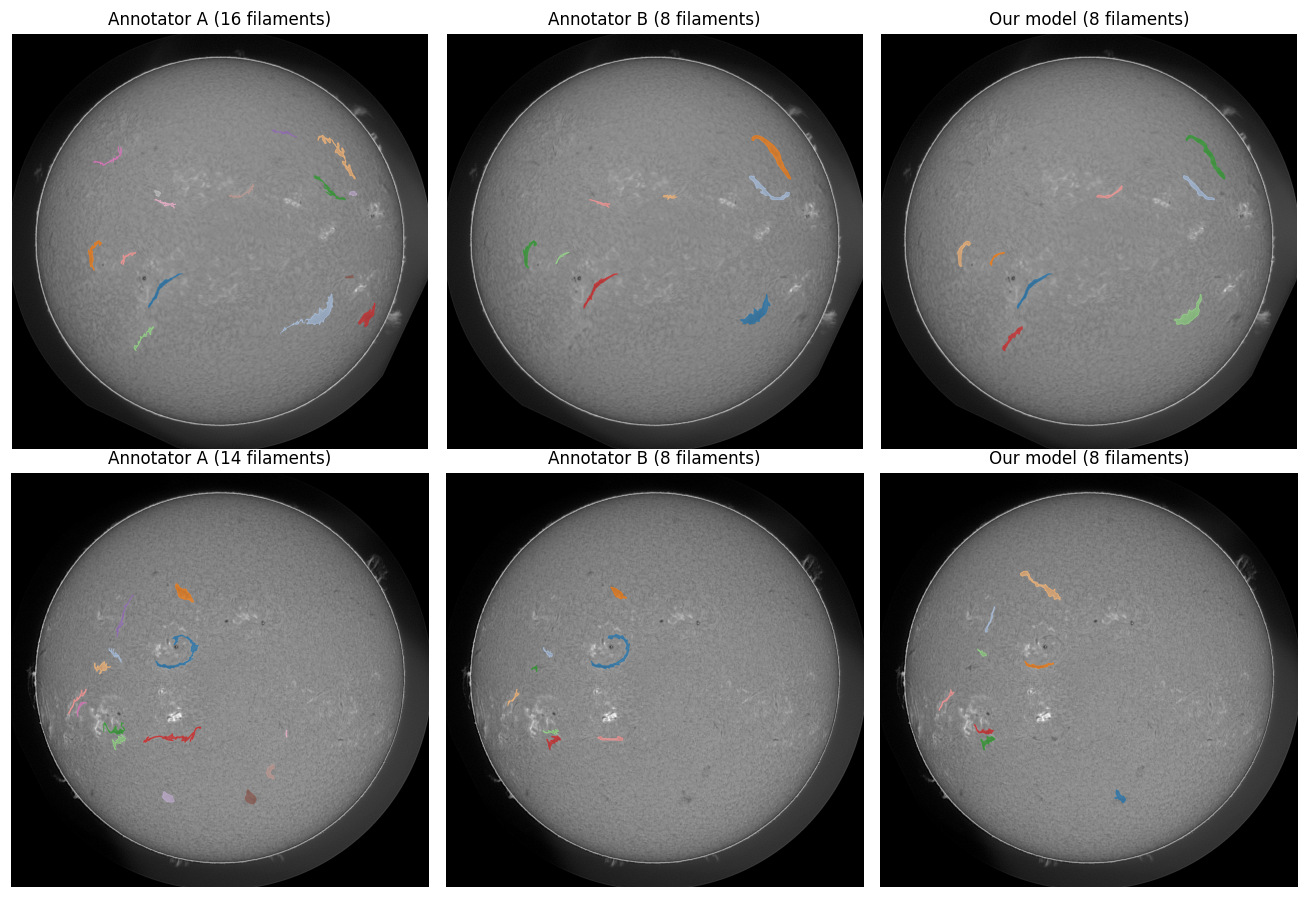
\includegraphics[width=0.92\textwidth]{fig_examples.png}
  \vspace{-3mm}
  \caption{Two held-out observations, each annotated by two experts (left, middle), and our prediction (right). In both, annotator~A marks 14--16 filaments and annotator~B only~8; many of A's extra filaments are small.}
  \label{fig:examples}
\end{figure*}


% ==================================== %
%              EVALUATION              %
% ==================================== %
\section{Evaluation}\label{sec:evaluation}

\subsection{Strategy}
We score held-out predictions with the organizers' PQ definition \cite{kirillov2019panoptic}: a pair is a true positive when IoU $>$0.5, ground truth is grouped per annotator pass, and predictions per observation. Our implementation follows the organizers' self-evaluation notebook but works on RLEs. Uncertainty is a 95\% bootstrap interval over the 106 held-out observations \cite{efron1979bootstrap} (2{,}000 resamples; paired when comparing variants) and a Wilson interval for recalls \cite{wilson1927}. For the three pipelines we scored both ways, held-out PQ ranked them in the same order as the public leaderboard, 0.04--0.06 higher.

\subsection{Results}
\begin{table}[t]
  \caption{Held-out PQ (95\% CI) and public leaderboard (LB). Upper part: the path to the final pipeline; lower part: variants we tried and did not adopt (best score threshold for each).}
  \label{tab:ablation}
  \small
  \setlength{\tabcolsep}{3pt}
  \begin{tabular}{lccc}
    \toprule
    Variant & PQ & TP/FP/FN & LB \\
    \midrule
    Public notebook \cite{gluhkikh2026notebook} & 0.409 {\scriptsize[.384,.434]} & 752/476/506 & 0.37 \\
    Ours, 1280 det., nearest upsampling & 0.423 & 707/297/551 & -- \\
    \ \ + flip TTA, linear upsampling, LCC & 0.437 & 720/288/538 & 0.38$^\dagger$ \\
    \ \ + WBF with 1920 det. (\textbf{final}) & \textbf{0.444} {\scriptsize[.419,.467]} & 750/326/508 & \textbf{0.39} \\
    \midrule
    1920 detector alone & 0.433 & 746/374/512 & \\
    YOLO11m, 120 epochs & 0.423 & 741/403/517 & \\
    YOLO11s, 120 epochs, new seed & 0.427 & 755/418/503 & \\
    WBF of four detectors & 0.441 & 732/311/526 & \\
    Detector test-time augmentation & 0.432 & 757/391/501 & \\
    Refiner with clDice loss \cite{shit2021cldice} & 0.437 & 746/335/512 & \\
    Masks dilated by 1 px$^\ddagger$ & 0.392 & 734/493/524 & \\
    Masks eroded by 2 px$^\ddagger$ & 0.230 & 455/705/803 & \\
    \bottomrule
  \end{tabular}\\[2pt]
  {\scriptsize $^\dagger$submitted at score threshold 0.28 (held-out 0.436). $^\ddagger$applied to the public-notebook predictions.}
\end{table}

Table~\ref{tab:ablation} summarizes the measurements. The final pipeline improves on the public reference by +0.035 PQ (paired 95\% CI +0.022 to +0.047). The step from one to two fused detectors is +0.008 and \emph{not} significant (CI $-$0.001 to +0.018); we keep it because it was the better variant at every score threshold from 0.24 upward. The free inference changes in Stage~2 (flip TTA, linear instead of nearest upsampling, largest component) gave +0.014, mostly from the upsampling. Larger or longer-trained detectors, detector TTA, four-detector fusion and a skeleton-aware loss did not help.

Matched pairs have a mean IoU of 0.69 and a mean Dice of 0.81 (Fig.~\ref{fig:results}b). Counting every overlap (IoU $>$0) as in the organizers' notebook, 855 ground-truth filaments overlap exactly one prediction, 78 overlap several (fragmentation), and 325 none; 952 predictions overlap one filament, 35 several (over-merging), and 89 none. Over-merging and fragmentation are therefore minor; missed filaments dominate.

\begin{figure}[t]
  \centering
  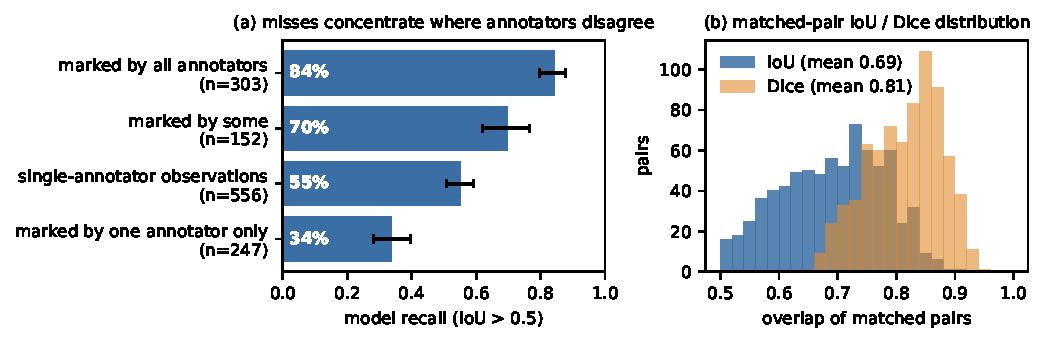
\includegraphics[width=\columnwidth]{fig_results.pdf}
  \vspace{-6mm}
  \caption{(a) Recall of the final pipeline on held-out filaments, grouped by how many annotators of the same observation marked them (95\% Wilson intervals). (b) IoU and Dice of matched pairs.}
  \label{fig:results}
\end{figure}

\subsection{Where the errors are: annotator disagreement}
Forty of the 106 held-out observations have two or more annotator passes. Scoring one annotator's masks against the other annotators of the same observation, as if they were predictions, gives PQ 0.33 with a mean matched IoU of 0.63: human annotators agree with each other less than our model agrees with them (0.44).

We grouped every ground-truth filament on these observations by how many of the \emph{other} annotators also marked it (IoU $>$0.5). Figure~\ref{fig:results}a shows the result: the model finds 84\% of the filaments marked by all annotators, 70\% of those marked by some, and only 34\% of those marked by a single annotator; the last group is also smaller (median 1{,}157 vs 1{,}663~px). Conversely, of the 213 predictions that count as false positives against one annotator, 112 (53\%) were drawn by another annotator of the same image.

To separate detection from mask quality we fed the refiner the ground-truth boxes instead of detector boxes. PQ rises from 0.44 to 0.60, and on single-annotator observations the refiner then recovers 545 of 556 filaments with a mean IoU of 0.72, above the 0.63 inter-annotator IoU. Mask shape is thus at human level; the remaining gap is about \emph{which} faint, small structures count as filaments, a decision on which the experts themselves differ.

\subsection{Strengths, weaknesses and improvements}
\textbf{Strengths.} The pipeline is fast, deterministic, strictly non-overlapping, and reproduces its submission byte-for-byte; on consensus filaments its recall is 84\%.
\textbf{Weaknesses.} Recall on small, faint filaments is low; masks are sensitive to their boundary (a 1~px dilation already costs 0.017 PQ, a 2~px erosion 0.18), which also explains why our earlier global 512~px semantic model scored only 0.29 on the leaderboard; one test observation receives no instance.
\textbf{Improvements.} Training on consensus-weighted targets (e.g., soft labels from the number of annotators who marked a filament) instead of treating every pass as equally correct, and calibrating the detector's confidence to annotator agreement. For evaluation we suggest reporting recall stratified by annotator agreement next to PQ, and PQ relative to the inter-annotator ceiling; both are cheap to compute and make scores comparable across datasets with different labelling conventions.


% ==================================== %
%            ACKNOWLEDGMENT            %
% ==================================== %
\section{Acknowledgment}\label{sec:acknowledgment}
    % Do not change
    The organization of the Filament Segmentation Challenge 2026 is partially supported by the U.S. National Science Foundation (NSF) under Grant No. 2209912 and 2433781, directorate for Computer and Information Science and Engineering (CSE), and Office of Advanced Cyberinfrastructure (OAC), and Grant No. 2511630, AST Division Of Astronomical Sciences and MPS Directorate for Mathematical and Physical Sciences.

    The Filament Segmentation Challenge 2026 is sponsored by the U.S. National Science Foundation (NSF) National Solar Observatory (NSO).

    This work utilizes GONG data obtained by the NSO Integrated Synoptic Program, managed by the National Solar Observatory, which is operated by the Association of Universities for Research in Astronomy (AURA), Inc. under a cooperative agreement with the National Science Foundation and with contribution from the National Oceanic and Atmospheric Administration. The GONG network of instruments is hosted by the Big Bear Solar Observatory, High Altitude Observatory, Learmonth Solar Observatory, Udaipur Solar Observatory, Instituto de Astrofísica de Canarias, and Cerro Tololo Interamerican Observatory.

\bibliographystyle{ACM-Reference-Format}
\bibliography{main}

\end{document}
